%iffalse
\let\negmedspace\undefined
\let\negthickspace\undefined
\documentclass[journal,12pt,onecolumn]{IEEEtran}
\usepackage{cite}
\usepackage{amsmath,amssymb,amsfonts,amsthm}
\usepackage{algorithmic}
\usepackage{graphicx}
\usepackage{textcomp}
\usepackage{xcolor}
\usepackage{txfonts}
\usepackage{listings}
\usepackage{enumitem}
\usepackage{mathtools}
\usepackage{gensymb}
\usepackage{comment}
\usepackage[breaklinks=true]{hyperref}
\usepackage{tkz-euclide} 
\usepackage{listings}
\usepackage{gvv}                                        
\def\inputGnumericTable{}                                 
\usepackage[latin1]{inputenc}                                
\usepackage{color}                                            
\usepackage{array}                                             
\usepackage{longtable}                                       
\usepackage{calc}                                             
\usepackage{multirow}                                         
\usepackage{hhline}                                           
\usepackage{ifthen}                                           
\usepackage{lscape}
\usepackage{multicol}

\newtheorem{theorem}{Theorem}[section]
\newtheorem{problem}{Problem}
\newtheorem{proposition}{Proposition}[section]
\newtheorem{lemma}{Lemma}[section]
\newtheorem{corollary}[theorem]{Corollary}
\newtheorem{example}{Example}[section]
\newtheorem{definition}[problem]{Definition}
\newcommand{\BEQA}{\begin{eqnarray}}
\newcommand{\EEQA}{\end{eqnarray}}
\newcommand{\define}{\stackrel{\triangle}{=}}
\theoremstyle{remark}
\newtheorem{rem}{Remark}
\begin{document}

\bibliographystyle{IEEEtran}
\vspace{3cm}

\title{NCERT - 10.4.ex.4}
\author{EE224BTECH11044 - Muthyala koushik
}
\maketitle
\bigskip

\renewcommand{\thefigure}{\theenumi}
\renewcommand{\thetable}{\theenumi}
\textbf{\section{QUADRATIC EQUATIONS}}

\textbf{Question:} Find the roots of the quadratic equation $3x^2 - 2\sqrt{6}x + 2 = 0$ \\ 
\solution The given equation:
\begin{align}
	3x^2-2\sqrt{6}x+2 &= 3x^2-\sqrt{6}x-\sqrt{6}x+2	\\
	&=\sqrt{3}x\brak{\sqrt{3}x-\sqrt{2}}-\sqrt{2}\brak{\sqrt{3}x-\sqrt{2}}\\
	&=\brak{\sqrt{3}x-\sqrt{2}}\brak{\sqrt{3}x-\sqrt{2}}
\end{align}

So, the roots of the equation are the values of x for which
\begin{align}
	\brak{\sqrt{3}x-\sqrt{2}}\brak{\sqrt{3}x-\sqrt{2}}&=0\\
	\sqrt{3}x-\sqrt{2}&=0\\
	x&=\sqrt{\frac{2}{3}}
\end{align}

Therefore, the roots of $3x^2 - 2\sqrt{6}x + 2 = 0$ are $\sqrt{\frac{2}{3}}$, $\sqrt{\frac{2}{3}}$\\

\textbf{Solution by the method of Fixed point Iteration}\\
Rearrange the equation to $x=g\brak{x}$
\begin{align}
	x=\frac{1}{3}\brak{2\sqrt{6}-\frac{2}{x}}
\end{align}

This gives the iteration function:
\begin{align}
	g\brak{x}=\frac{1}{3}\brak{2\sqrt{6}-\frac{2}{x}}
\end{align}

Iteration: Use the formula repeatedly:
\begin{align}
	x_{n+1}=\frac{1}{3}\brak{2\sqrt{6}-\frac{2}{x_n}}
\end{align}

Stop when $\abs{x_{n+1}-x_n}<\epsilon$\\
Root: 0.8173993362392574, Iterations: 900\\
Actual Root:0.81649658092\\


\textbf{Solution by the Newton-Raphson method:}
we have;
\begin{align}
	x_{n+1}&=x_n -\frac{f\brak{x_n}}{f^{'}\brak{x_n}}\\
	x_{n+1}&=x_n - \frac{3x^2 - 2\sqrt{6}x + 2}{6x - 2\sqrt{6}x}
\end{align}

Iterating and updating the value of $x_{n}$, we can obtain the roots of the quadratic equation. \\
Newton-Raphson Root: 0.8164972809158475, Iterations: 18\\
Actual Root:0.81649658092\\

\begin{figure}[h]
	\centering
	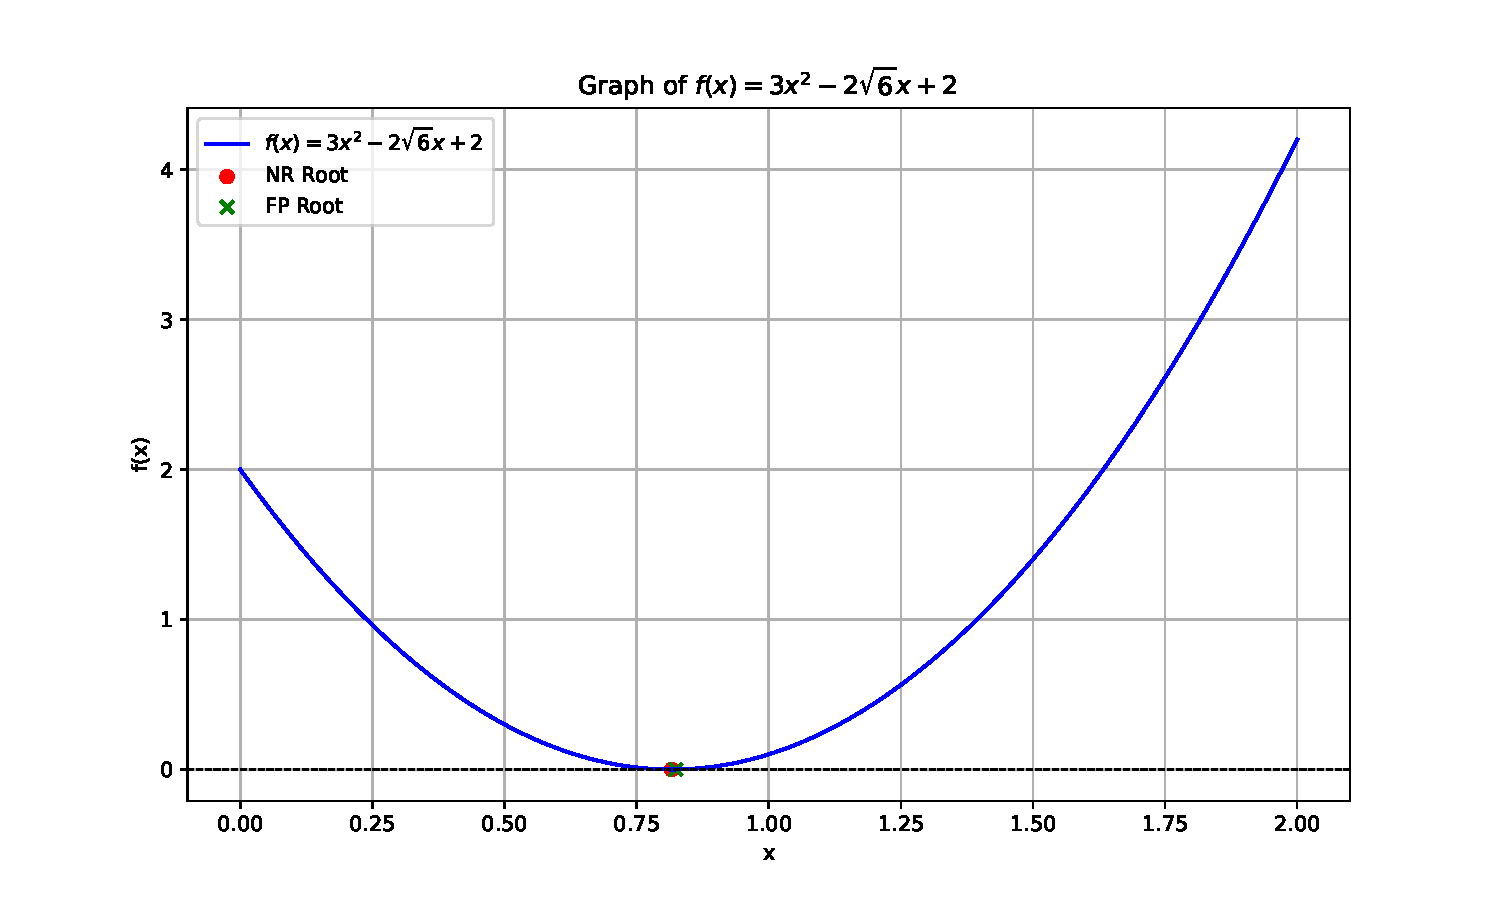
\includegraphics[width=\columnwidth]{figs/fig.pdf}
	\caption{Solution of given DE}
	\label{fig}
\end{figure}

\end{document}
